\documentclass[11pt,a4paper]{ltjsarticle}

\usepackage{amsmath}
\usepackage{graphicx}
\usepackage{booktabs}
\usepackage{geometry}
\usepackage{siunitx}
\usepackage{hyperref}

\geometry{margin=25mm}

\title{演奏制御システムにおける\\Master Arduino → Slave Processing 間遅延の定量計測}
\author{グループ7}
\date{\today}

\begin{document}
\maketitle

\section{目的}
本システムは Master Arduino（以下 MA）が全体のテンポ（BPM）を管理し，
I2C経由で各楽器の Slave Arduino（以下 SA）へ Tick 信号をブロードキャストし，
SA は受信した Tick に応じて楽譜データを計算し，Serial経由で
対応する Slave Processing（以下 SP）に音符情報を送信して実際の音を再生する，
という多段構成になっている。

本レポートは，MAがBPM Tickを送信してから，対応する楽器（ピアノ）の音が
SPで再生されるまでの遅延を定量的に計測し，シリアル通信のボーレートが
遅延に与える影響を評価することを目的とする。

\section{システム構成}
測定対象の信号経路を図\ref{fig:architecture}に示す。

\begin{figure}[h]
\centering
\fbox{\parbox{0.9\linewidth}{\centering
\vspace{4mm}
\textbf{MasterProcessing} (UI.pde)
$\xrightarrow{\text{Serial}}$
\textbf{Master Arduino (MA)}
$\xrightarrow{\text{I2C broadcast}}$
\textbf{Slave Arduino (SA, ピアノ)}
$\xrightarrow{\text{Serial}}$
\textbf{SlaveProcessing} (SP\_Piano.pde)
$\rightarrow$ 音声出力
\vspace{4mm}
}}
\caption{計測対象の信号経路}
\label{fig:architecture}
\end{figure}

MAは一定間隔（$15000/\mathrm{BPM}$ [ms]）でBPM Tickを全Slaveへブロードキャストし，
SAはTickを受信するたびに楽譜中の該当インデックスの音高・長さを計算してSPへ送信する。
SPはこれを受信し，Minimライブラリで実際に音を再生する。

\section{計測手法}

\subsection{計測の基本方針}
\begin{itemize}
  \item 本番用コード（\texttt{group7/FINAL}）は変更せず，計測専用に複製した
        \texttt{group7/TEST} 環境で計測を行った。
  \item SA→SPのシリアルプロトコルに，計測専用の一時的な「Tick番号」フィールドを
        追加し，MA側が送信したTick番号とSP側の受信イベントを1対1で対応付けられるようにした。
  \item MasterProcessingは，MAが出力するTick送信ログを受信した時刻を，
        SlaveProcessing（ピアノ）は音符データを受信・再生した時刻を，
        それぞれミリ秒精度でCSVファイルに記録した。
  \item MAとSAを同一PCに接続し，両Processingスケッチを同一マシン上で動作させることで，
        複数PC間のクロック同期の問題を回避し，同一のOS時計上で時刻比較を行えるようにした。
\end{itemize}

\subsection{遅延の算出方法}
計測後，MA側のTick送信ログ（Tick番号と受信時刻）と，SP側の受信・再生ログ
（Tick番号と受信時刻）の2つのCSVファイルをTick番号でJOINし，
\[
  \mathrm{delay} = T_{\mathrm{SP\,recv}} - T_{\mathrm{MA\,log\,recv}}
\]
として各Tickごとの遅延を算出した。休符（音を伴わないTick）は集計対象から除外し，
実際に音が発生したイベントのみを評価対象とした。

\subsection{計測条件}
対象楽器はピアノ。BPMとシリアル通信のボーレートを変えた4条件で計測した。

\begin{table}[h]
\centering
\caption{計測条件}
\begin{tabular}{lll}
\toprule
条件 & BPM & ボーレート [bps] \\
\midrule
条件A & 120 & 9600 \\
条件B & 180 & 9600 \\
条件C & 120 & 115200 \\
条件D & 180 & 115200 \\
\bottomrule
\end{tabular}
\end{table}

\subsection{評価基準}
遅延の大小は，以下の2つの基準で評価した。

\begin{table}[h]
\centering
\caption{絶対値基準（人間の知覚閾値に基づく）}
\begin{tabular}{ll}
\toprule
delay & 評価 \\
\midrule
20 ms 未満 & ほぼ知覚不可能 \\
20--50 ms & 許容範囲 \\
50--100 ms & 要注意 \\
100 ms 以上 & 問題あり \\
\bottomrule
\end{tabular}
\end{table}

\begin{table}[h]
\centering
\caption{相対値基準（Tick間隔 $=15000/\mathrm{BPM}$ [ms] に対する比率）}
\begin{tabular}{ll}
\toprule
delay / Tick間隔 & 評価 \\
\midrule
10\% 未満 & 全く問題なし \\
10--25\% & 許容範囲 \\
25--50\% & 要注意 \\
50\% 以上 & 致命的 \\
\bottomrule
\end{tabular}
\end{table}

\section{結果}

\subsection{統計量}
各条件における有効サンプル数は211件（対応するTickが見つからなかった件数は0件）であった。
統計量を表\ref{tab:stats}に示す。

\begin{table}[h]
\centering
\caption{条件別の遅延統計量}
\label{tab:stats}
\begin{tabular}{lrrrrrr}
\toprule
条件 & 平均 [ms] & 中央値 [ms] & 標準偏差 [ms] & 最小 [ms] & 最大 [ms] & Tick間隔比 \\
\midrule
9600bps, BPM120   &  9.4 &  9.0 & 2.7 &  3 & 15 &  7.5\% \\
9600bps, BPM180   &  9.4 &  9.0 & 2.5 &  3 & 16 & 11.3\% \\
115200bps, BPM120 & $-0.9$ & $-1.0$ & 1.2 & $-3$ & 2 & $-0.7\%$ \\
115200bps, BPM180 & $-1.0$ & $-1.0$ & 1.3 & $-4$ & 2 & $-1.1\%$ \\
\bottomrule
\end{tabular}
\end{table}

\subsection{条件別の比較}
図\ref{fig:bar}に4条件の平均delay（誤差棒は標準偏差）を，
図\ref{fig:ratio}にTick間隔に対する相対比率を示す。

\begin{figure}[h]
\centering
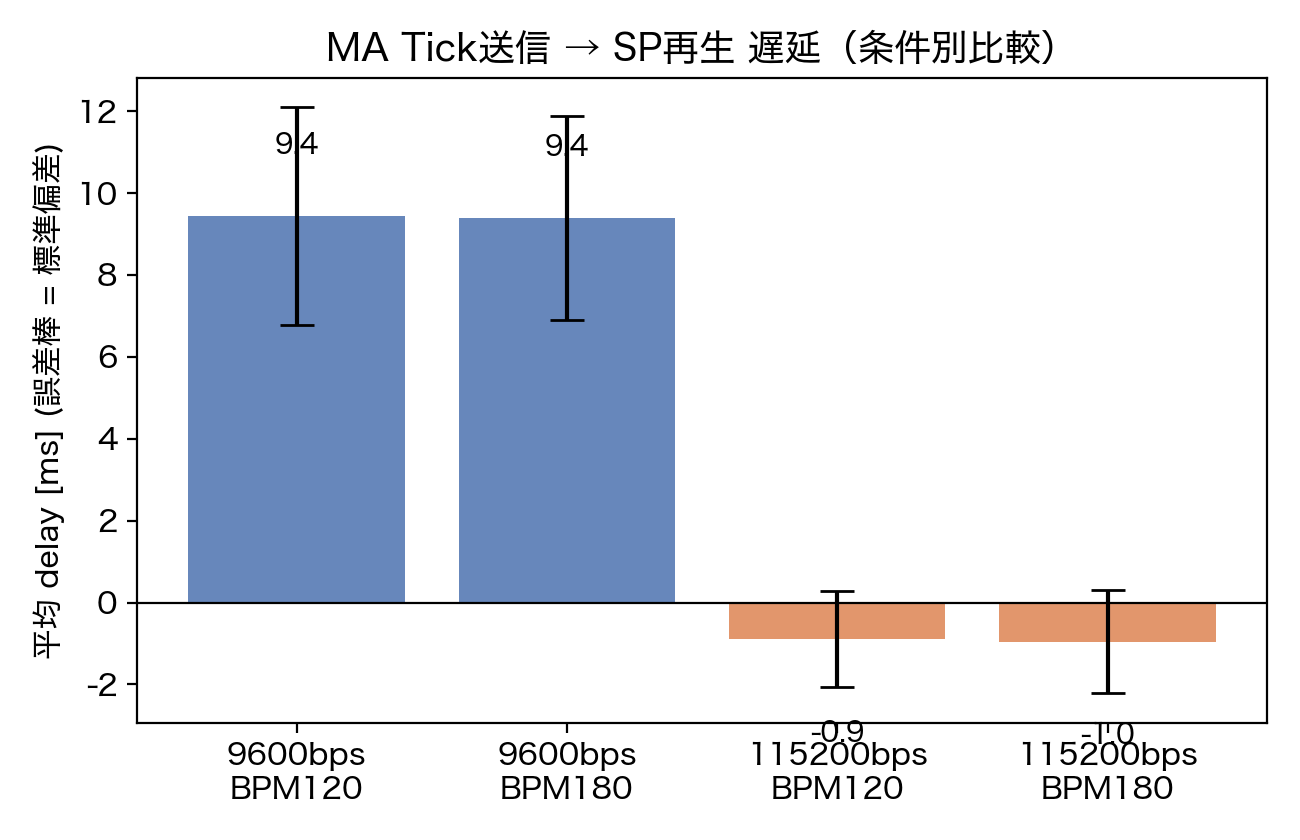
\includegraphics[width=0.75\linewidth]{fig_bar_comparison.png}
\caption{条件別の平均delay比較}
\label{fig:bar}
\end{figure}

\begin{figure}[h]
\centering
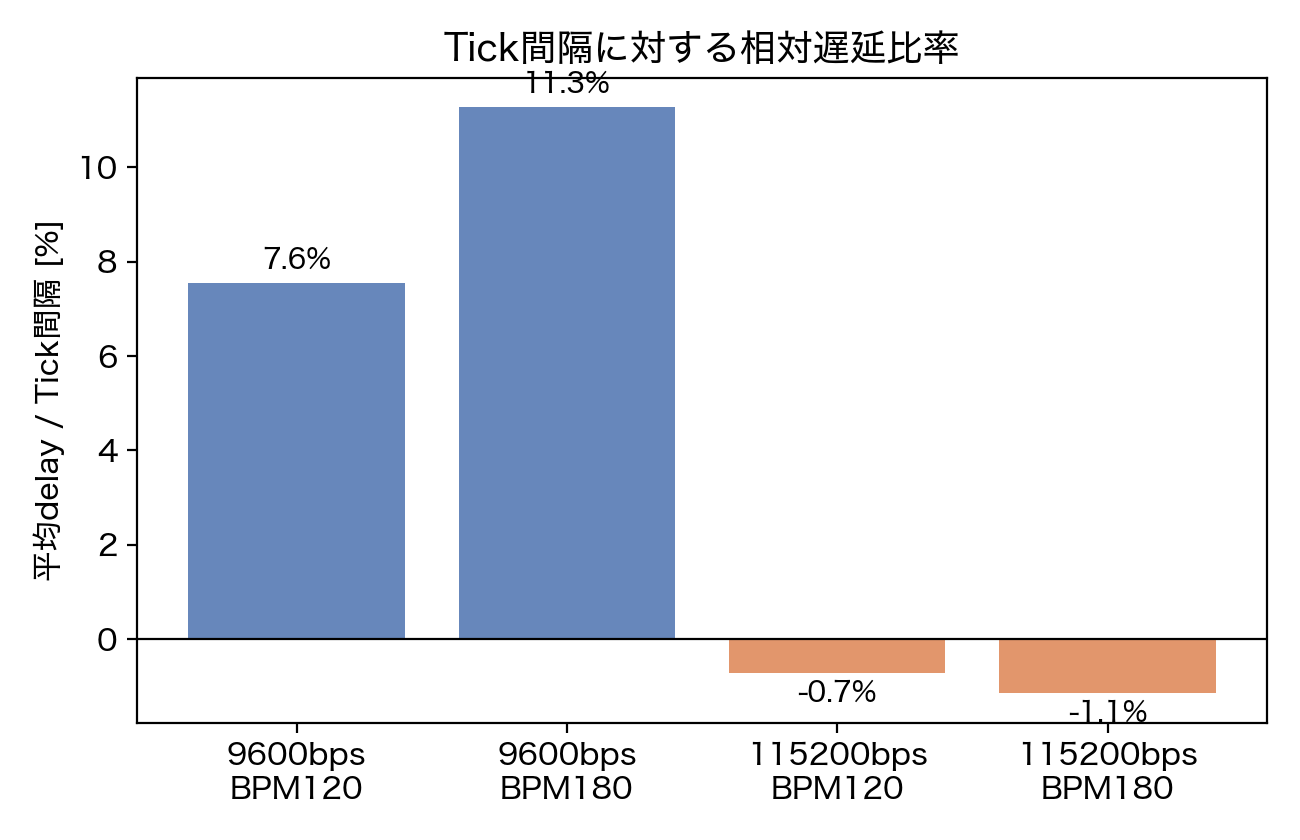
\includegraphics[width=0.75\linewidth]{fig_ratio.png}
\caption{Tick間隔に対する相対遅延比率}
\label{fig:ratio}
\end{figure}

\subsection{分布と時間的安定性}
図\ref{fig:hist}にBPM=120におけるdelayの分布（ボーレート別）を，
図\ref{fig:timeseries}にTick番号に対するdelayの推移を示す。
いずれのボーレートでも，演奏全体を通じてdelayが系統的に増大していく
ドリフトは見られず，値はそれぞれの分布の範囲内でランダムに揺れている。

\begin{figure}[h]
\centering
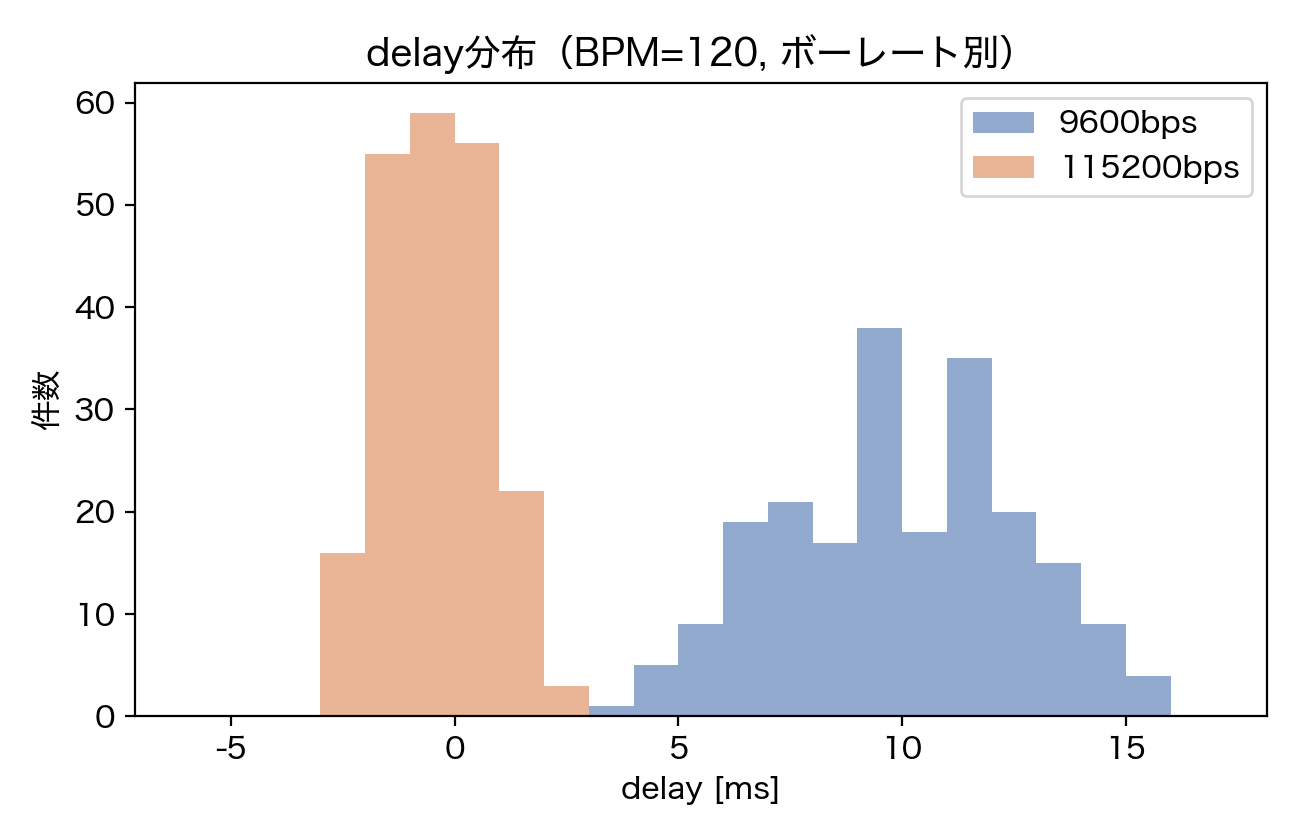
\includegraphics[width=0.75\linewidth]{fig_histogram.png}
\caption{delay分布（BPM=120，ボーレート別）}
\label{fig:hist}
\end{figure}

\begin{figure}[h]
\centering
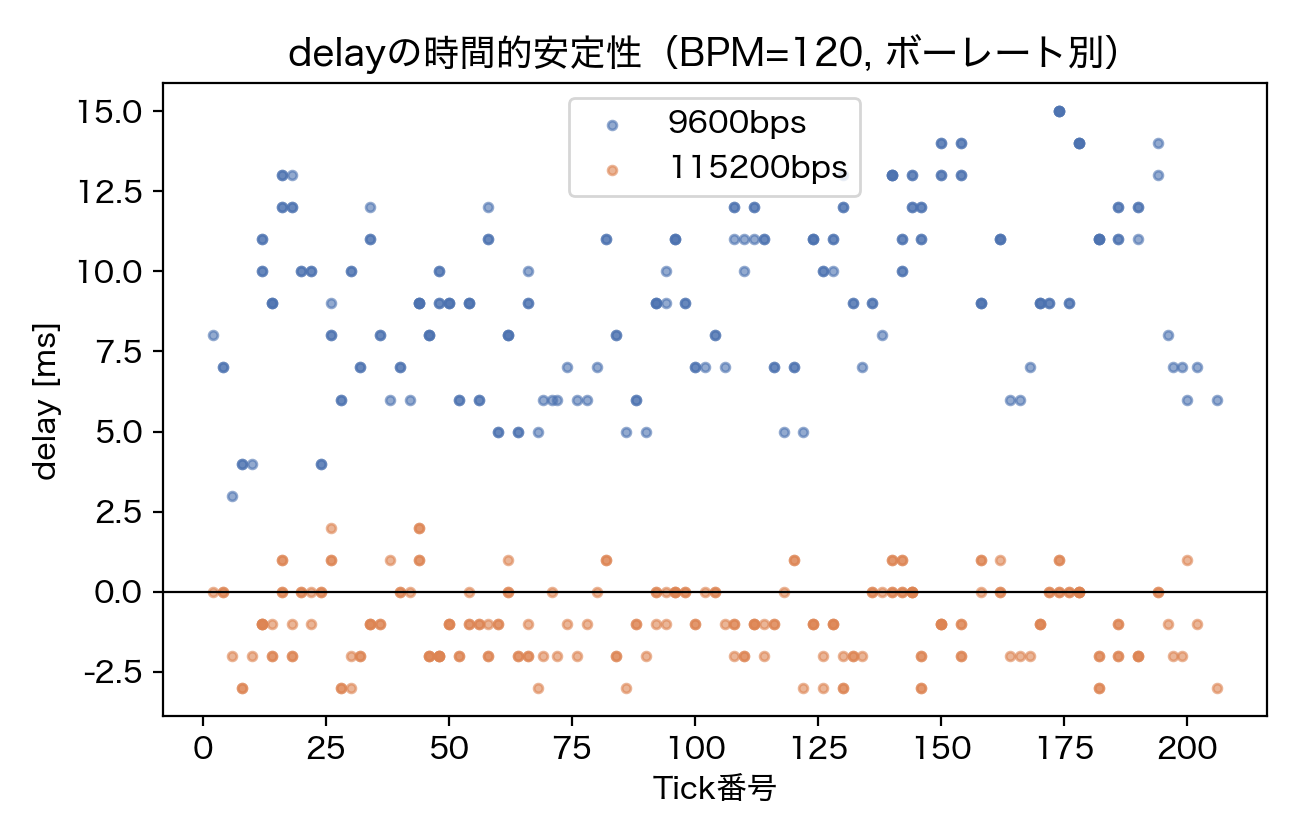
\includegraphics[width=0.75\linewidth]{fig_timeseries.png}
\caption{delayの時間的安定性（BPM=120，ボーレート別）}
\label{fig:timeseries}
\end{figure}

\section{考察}

\subsection{BPM依存性}
9600bpsの条件では，BPMを120から180に上げても平均delay（9.4ms）はほぼ変化しなかった。
これは，遅延の絶対値（ms）がBPMではなく，固定のシリアル通信速度に起因する
伝送時間によって決まっていることを示している。
一方，Tick間隔（$15000/\mathrm{BPM}$）はBPMの上昇に伴って縮小するため，
delayのTick間隔に対する相対比率は7.5\%から11.3\%に増加した。
すなわち，テンポが速くなるほど一定の絶対遅延が相対的に「厳しく」なる。

\subsection{ボーレートの影響}
ボーレートを9600bpsから115200bpsに上げたところ，平均delayは
約9.4msから約$-1$msまで縮小し，標準偏差も2.5--2.7msから1.2--1.3ms程度まで縮小した。
これは理論的な予測と一致する。本計測における「delay」は，
MA側のTick送信ログ（約30文字）とSA側の音符データ行（約13文字）という，
長さの異なる2つのシリアル行それぞれの伝送完了時刻の差分として定義されるため，
両者の伝送時間差そのものが測定値に系統的なバイアスとして乗っている。
9600bpsでは両者の伝送時間差は約18msと推定され，これが測定された約9.4msの
delayの主成分であったと考えられる。ボーレートを115200bpsに上げると
この伝送時間差は約1--2ms程度まで縮小し，測定されるdelayもほぼゼロ
（ノイズレベル）まで縮小する。115200bpsの条件でdelayがわずかに負の値を
取っているのは，この系統バイアスの符号が反転した結果であり，
実際の物理的な遅延が負になったことを意味するものではない。

\subsection{評価}
全4条件において，平均delayの絶対値は20ms未満（知覚閾値の許容範囲内），
Tick間隔に対する比率も最大で11.3\%（許容範囲：10--25\%）であり，
致命的な遅延は確認されなかった。特に115200bpsへの変更により，
シリアル通信起因の遅延はほぼ解消されることが確認できた。

\section{結論}
\begin{itemize}
  \item MA→SP間の遅延の絶対値はBPMに依存せず，シリアル通信のボーレートに
        起因する伝送時間が主要な決定因子であった。
  \item 9600bpsでは平均約9.4msの遅延が測定されたが，いずれの評価基準でも
        問題のないレベルであった。
  \item ボーレートを115200bpsに上げることで，シリアル伝送起因の遅延は
        ノイズレベルまで縮小し，さらなるマージンを確保できることを確認した。
  \item 本番反映の際は，関連する全ボード（MA・ピアノ・フルート・木琴・ドラム）と
        対応するProcessingスケッチのボーレートを統一して変更する必要がある。
\end{itemize}

\end{document}
